% #region PREAMBEL OG PAKKER
\documentclass[a4paper, 12pt]{article}  % DOKUMENTKLASSE
\title{IIK3100 -- Etisk hacking og penetrasjonstesting\\
[0.25em]Practical Assignment}           % TITTEL
\author{Kandidatnr: 10058}              % FORFATTER
\date{}                                 % DATO & FAG

\usepackage[english]{babel}             % SPRÅK
\usepackage[
    backend=biber,style=apa]{biblatex}  % BIBLIOGRAFI
\usepackage{csquotes}                   % PAKKE TIL BABEL
\addbibresource{bibliografi.bib}        % PATH TIL BIBLIOGRAFI
\usepackage[]{hyperref}                 % LENKER I TOC OG GENERELT
\usepackage[margin=1in]{geometry}       % VANLIG STØRRELSE MARGIN
\setlength{\parindent}{0em}             % SKILLER AVSNITT
\usepackage{graphicx}                   % BILDER \includegraphics[OPTIONS]{PATH}
\usepackage{kantlipsum}                 % FYLLTEKST I KANT-STIL (kant[n-m])
\usepackage{amsfonts,                   % BLACKBOARD BOLD FONT (\mathbb{N})
amsmath,stmaryrd,amssymb}               % ANDRE MATTE PAKKER
\usepackage{caption}                    % PAKKE FOR BEDRE CAPTIONS I FIGURER
\usepackage{float}                      % FLYTT FIGURER 
\usepackage[UTF8]{ctex}
\usepackage{alltt}
% #endregion
\includeonly{sections/getintouch}
\begin{document}
\newcounter{points}

\setlength{\parskip}{-0.25em}           % LINJEAVSTAND
\maketitle
\vspace{-4em}
\tableofcontents                        % INNHOLDSFORTEGNELSE
\thispagestyle{empty}
\addtocounter{page}{-1}
\setlength{\parskip}{.8em}              % LINJEAVSTAND

\section{OSINT}
\section{Technical information gathering}

\subsection{Spacex (30p)}
\addtocounter{points}{30}

Can you find the main SpaceX - Starlink ipv4 network range? Write it in CIDR format!

\textbf{Solution:}\\
For this task I looked up \url{starlink.com} on dnsdumpster and found an ip hosted from SpaceX - Starlink.

\begin{center}
    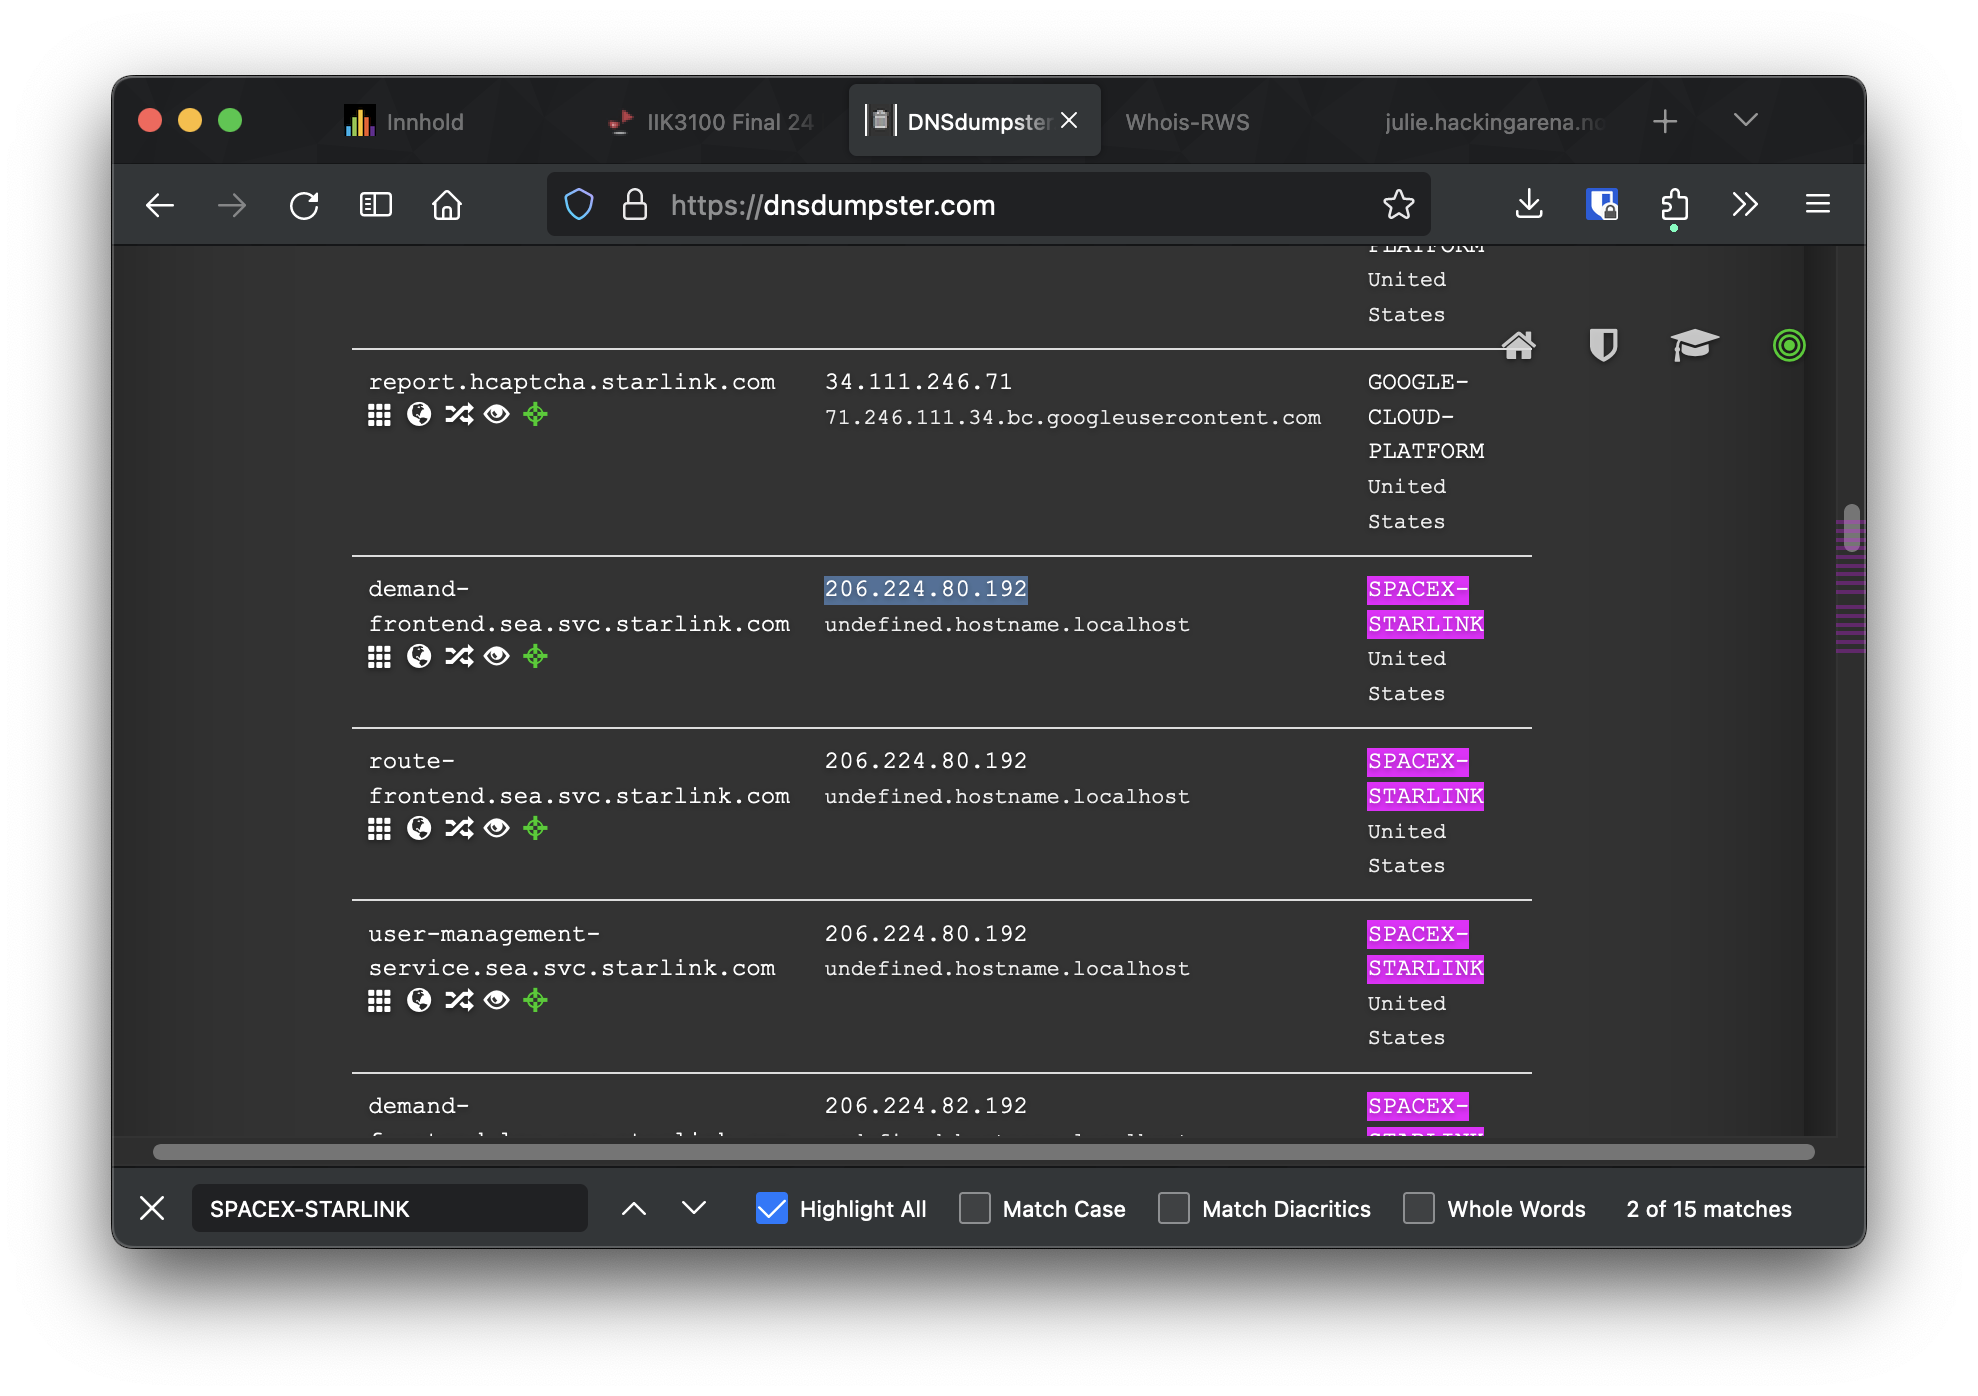
\includegraphics[width=12cm]{img/Technical information gathering/Spacex/Screenshot 2023-11-24 at 11.01.46.png}
\end{center}

After finding the ip I looked it up on ARIN and found the network range:

\begin{center}
    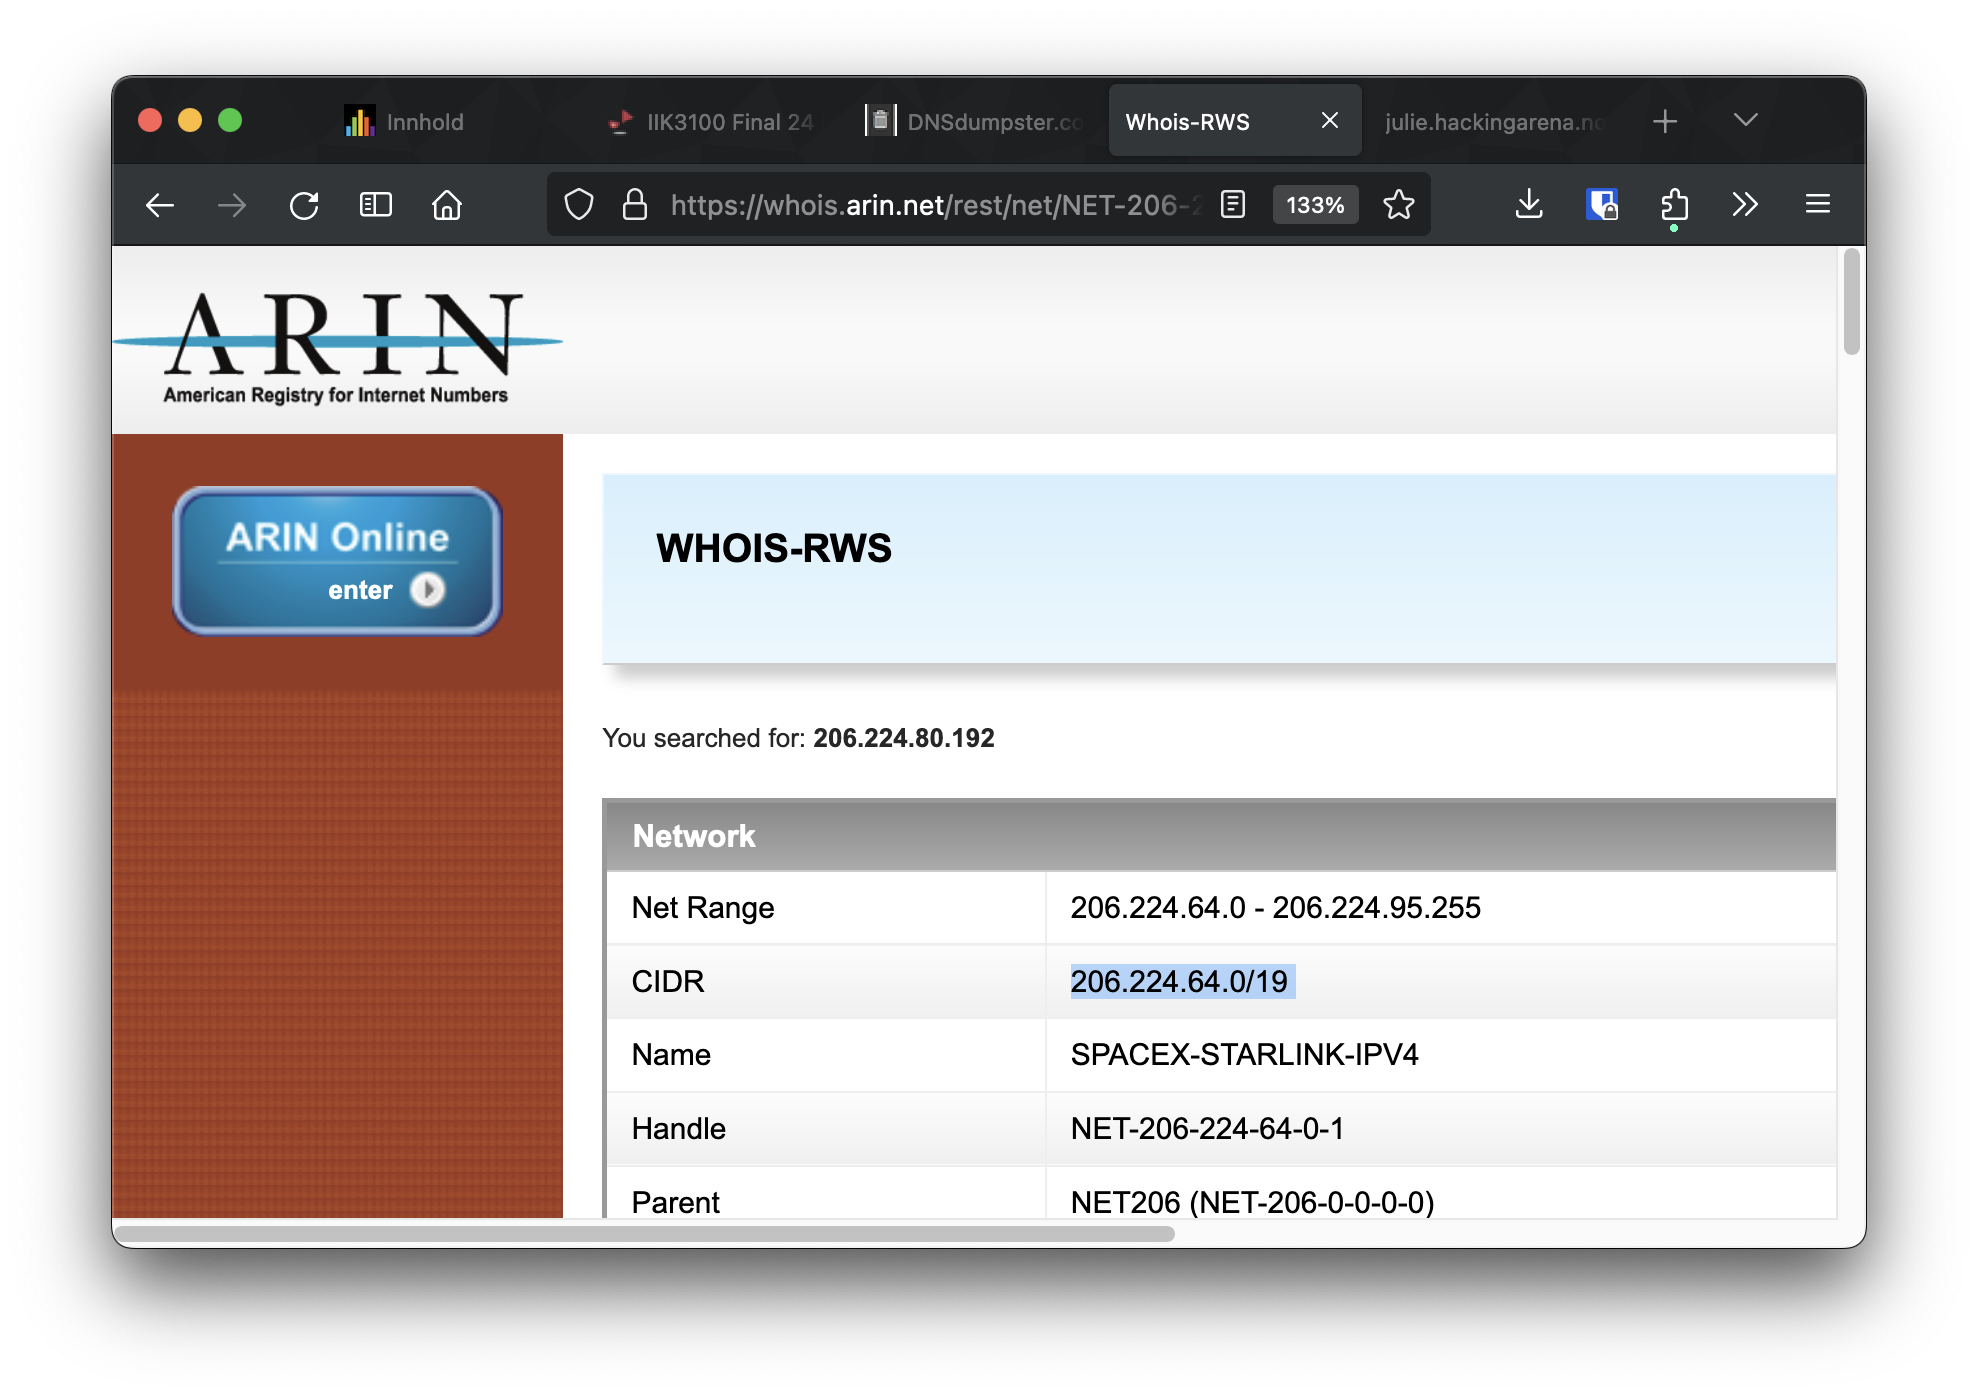
\includegraphics[width=11cm]{img/Technical information gathering/Spacex/Screenshot 2023-11-24 at 11.02.02.png}
\end{center}

\newpage
\subsection{Mysql in Lillesand (30p)}
\addtocounter{points}{30}
There are 3 mysql services available in Lillesand, can you find the ip of one of them?

Don't portscan anyone! Use only open source tools!

\textbf{Solution:}\\
For this task I used \url{search.censys.io} to search for mysql services located in Lillesand.

\begin{center}
    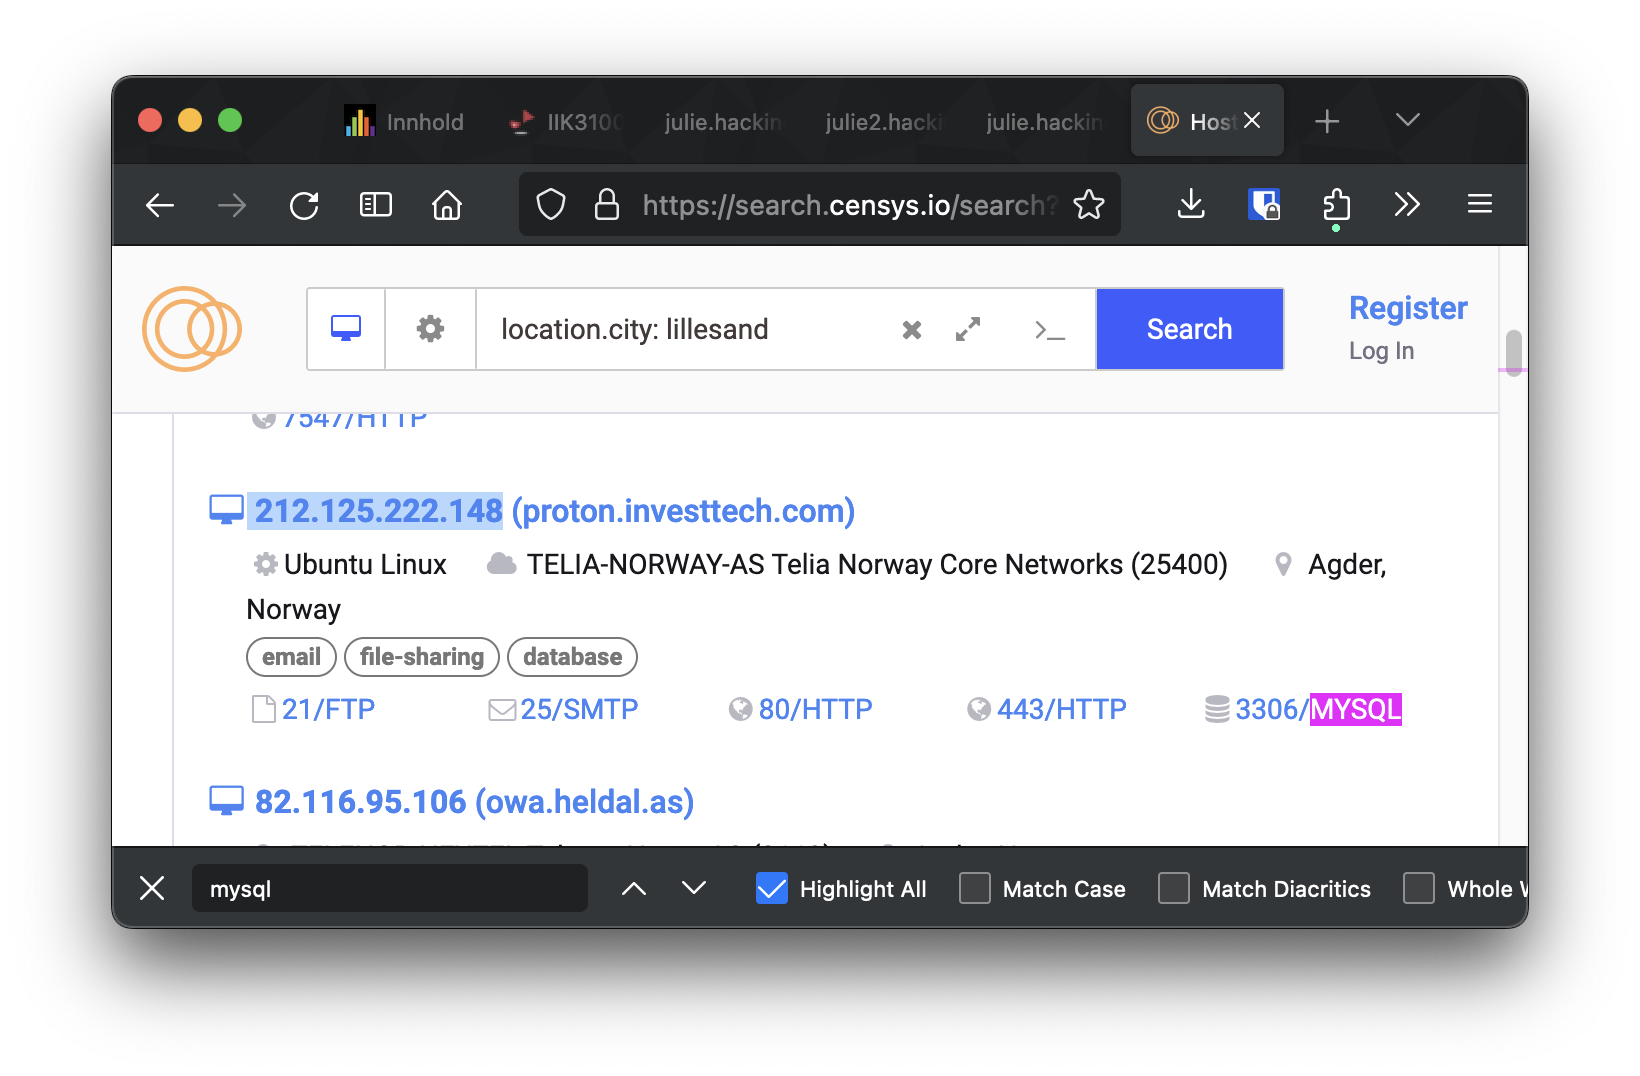
\includegraphics[width=15cm]{img/Technical information gathering/Mysql Lillesand/Screenshot 2023-11-24 at 11.16.26.png}
\end{center}
\section{Network mapping}

\subsection{Open ports (40p)}
\addtocounter{points}{40}
Check the open ports on julie2.hackingarena.no in the range 6000-7000. What is the sum of the open port numbers? If only port 6000 and 6001 are open, the answer is 12001.

\textbf{Solution:}\\
Using nmap I started a port scan using TCP connect on the range 6000 to 7000, and found four open ports.

\begin{center}
    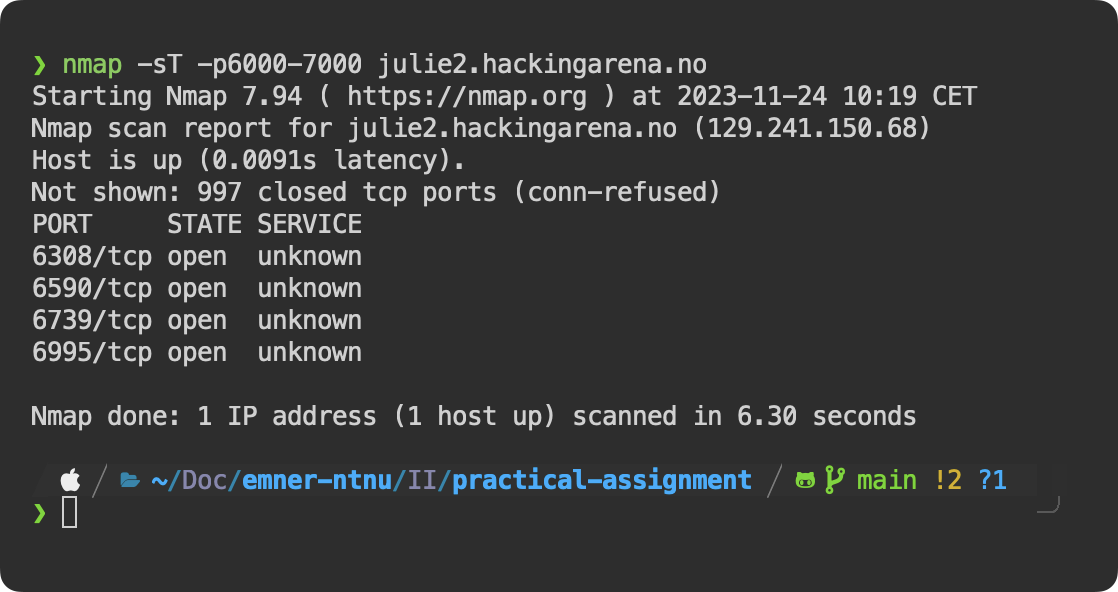
\includegraphics[width=15cm]{img/Network mapping/Open ports/Screenshot 2023-11-24 at 10.21.07.png}
\end{center}

Then adding the ports together I got the answer 26632.

\begin{center}
    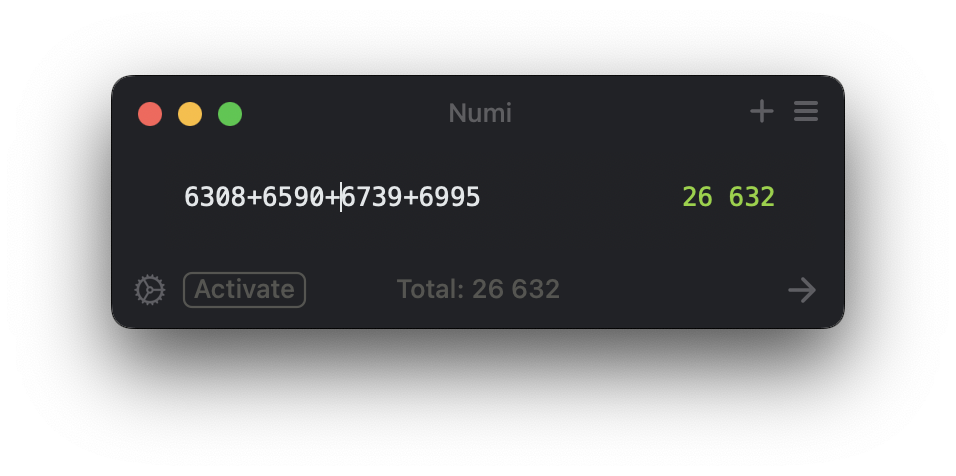
\includegraphics[width=15cm]{img/Network mapping/Open ports/Screenshot 2023-11-24 at 10.21.11.png}
\end{center}
\section{Hash cracking}

\subsection{Hash 1 (20p)}
\addtocounter{points}{20}
I do believe I'll be a tail fin hero on Norwegian in 50 years :) I travelled on a plane a few years ago, when I had to create my password, so I used the name on the tail. Here's the hash: 4b57b34a1855d0d9137d36023156717c What was my password?

\textbf{Solution:}\\
I first gathered a \href{https://en.wikipedia.org/wiki/List_of_Norwegian_Air_Shuttle_tail_fin_heroes_and_fleet}{list of the names of the people who are on the tail fin of Norwegian's planes}.

\begin{center}
    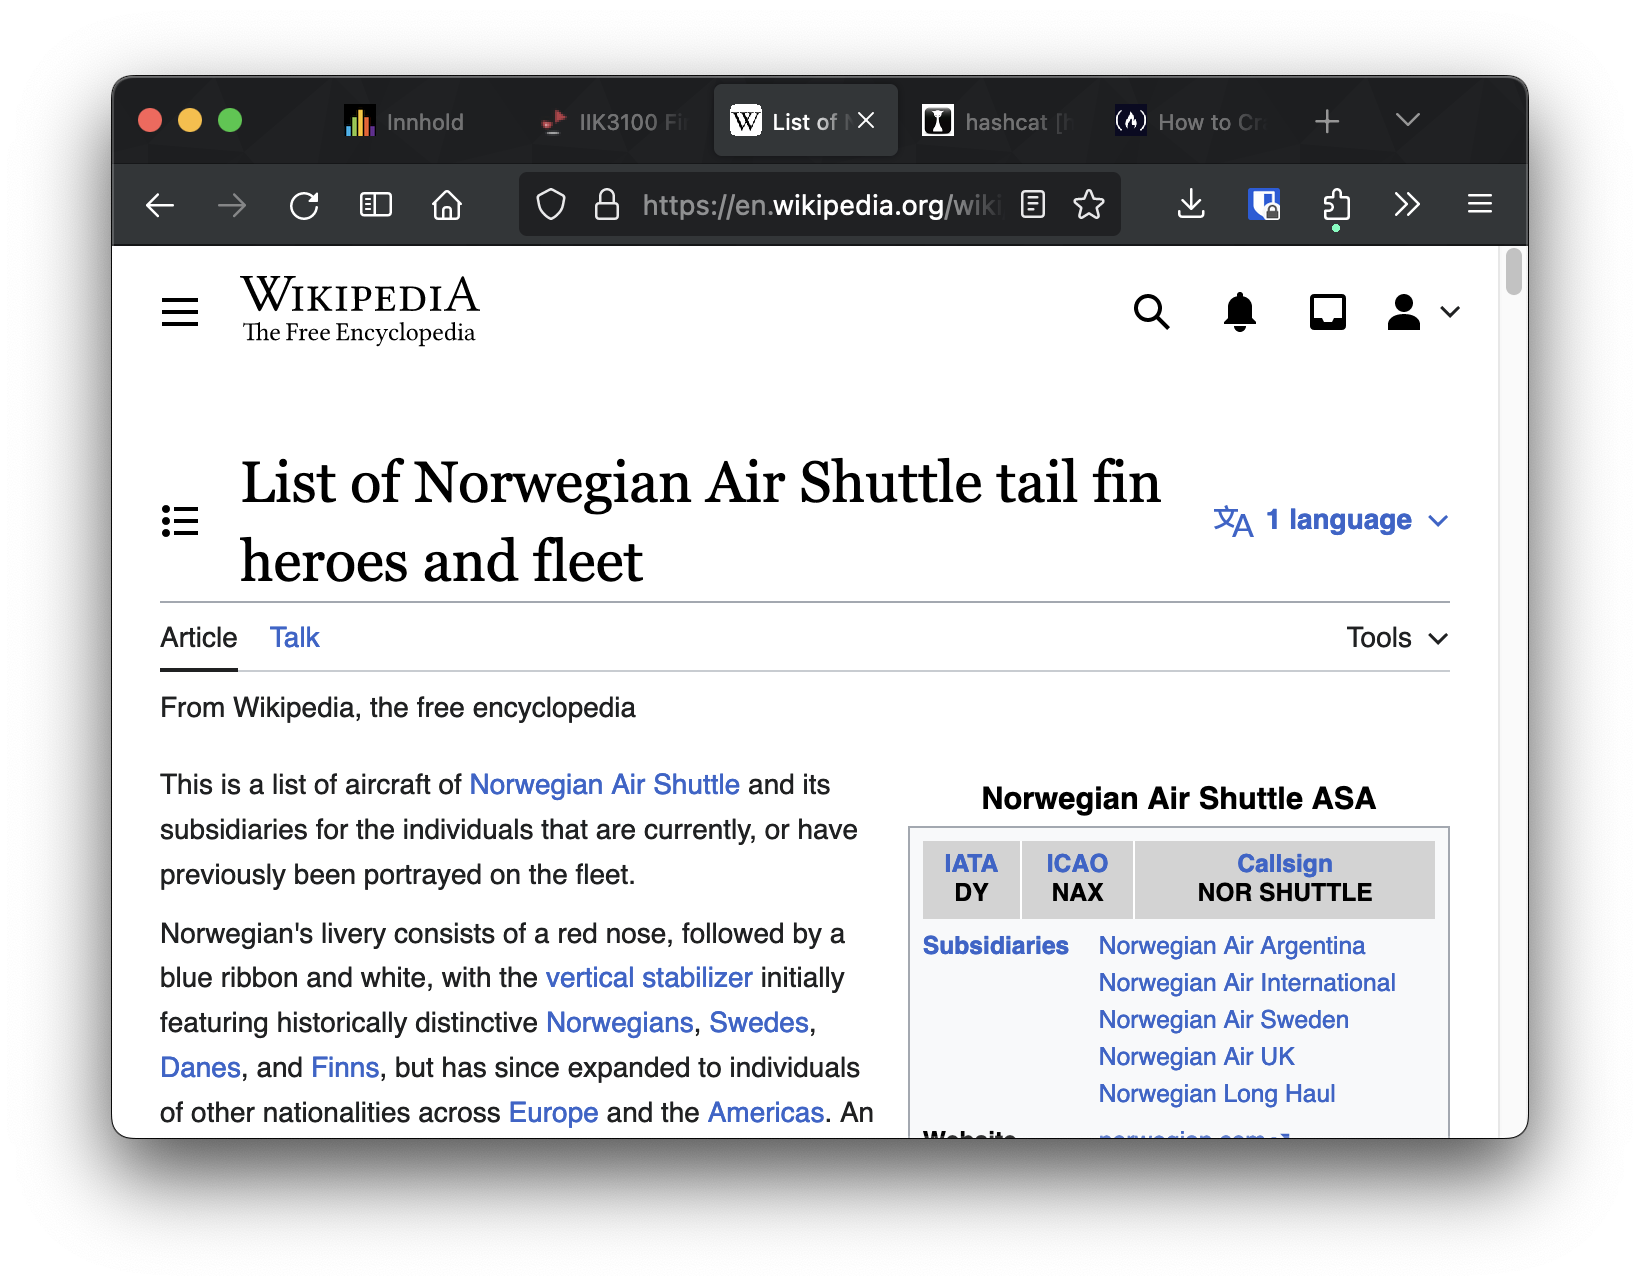
\includegraphics[width=10cm]{img/Hash cracking/Hash1/Screenshot 2023-11-24 at 10.47.35.png}
\end{center}

Then using hashcat I cracked the hash using the wordlist I created from the list of names.

\begin{center}
    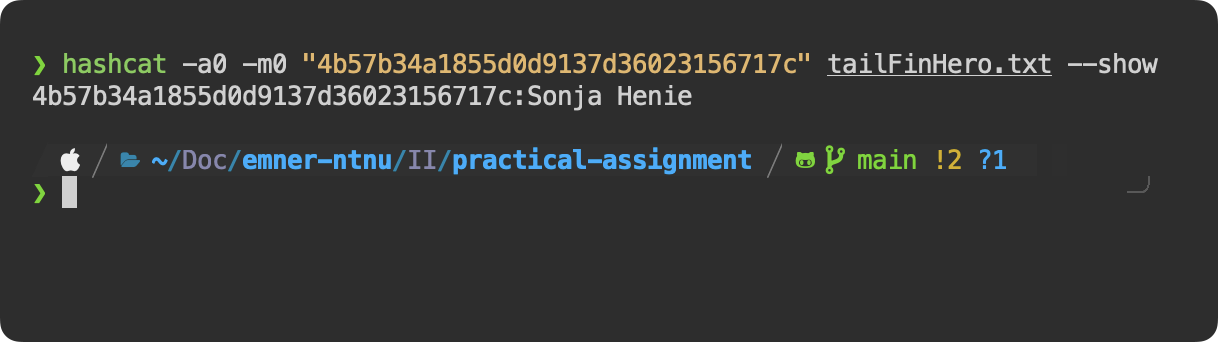
\includegraphics[width=15cm]{img/Hash cracking/Hash1/Screenshot 2023-11-24 at 10.46.31.png}
\end{center}
\section{Get in touch with services}

\subsection{5th challenge (80p)}
\addtocounter{points}{80}
Ladies and gentlemen, this is the 5th challenge.
\\A little bit of everything...
\\\url{julie.hackingarena.no} port 21000-21500

\textbf{Solution:}\\
First I ran a nmap port scan on the ports 21000-21500, and found a service running on port 21214. I also connected to the service using netcat and found that it was an FTP server.

\begin{center}
    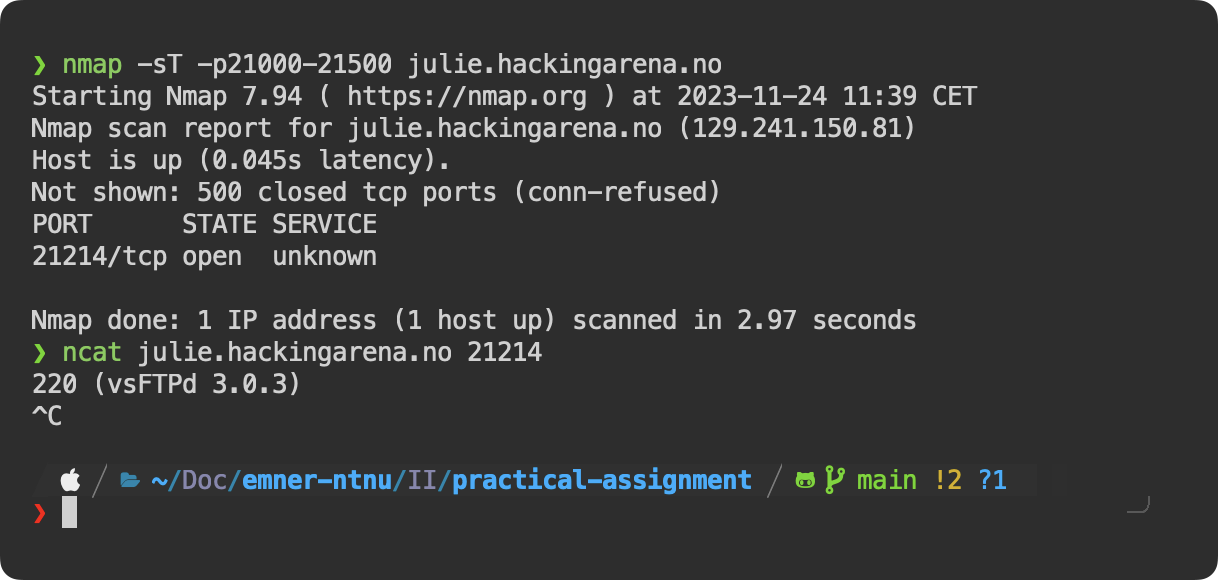
\includegraphics[width=11cm]{img/Get in touch with services/5th challenge/Screenshot 2023-11-24 at 14.23.03.png}
\end{center}

I then connected to the FTP server annonymously with filezilla and found six files named \texttt{shadow.old}.

\begin{center}
    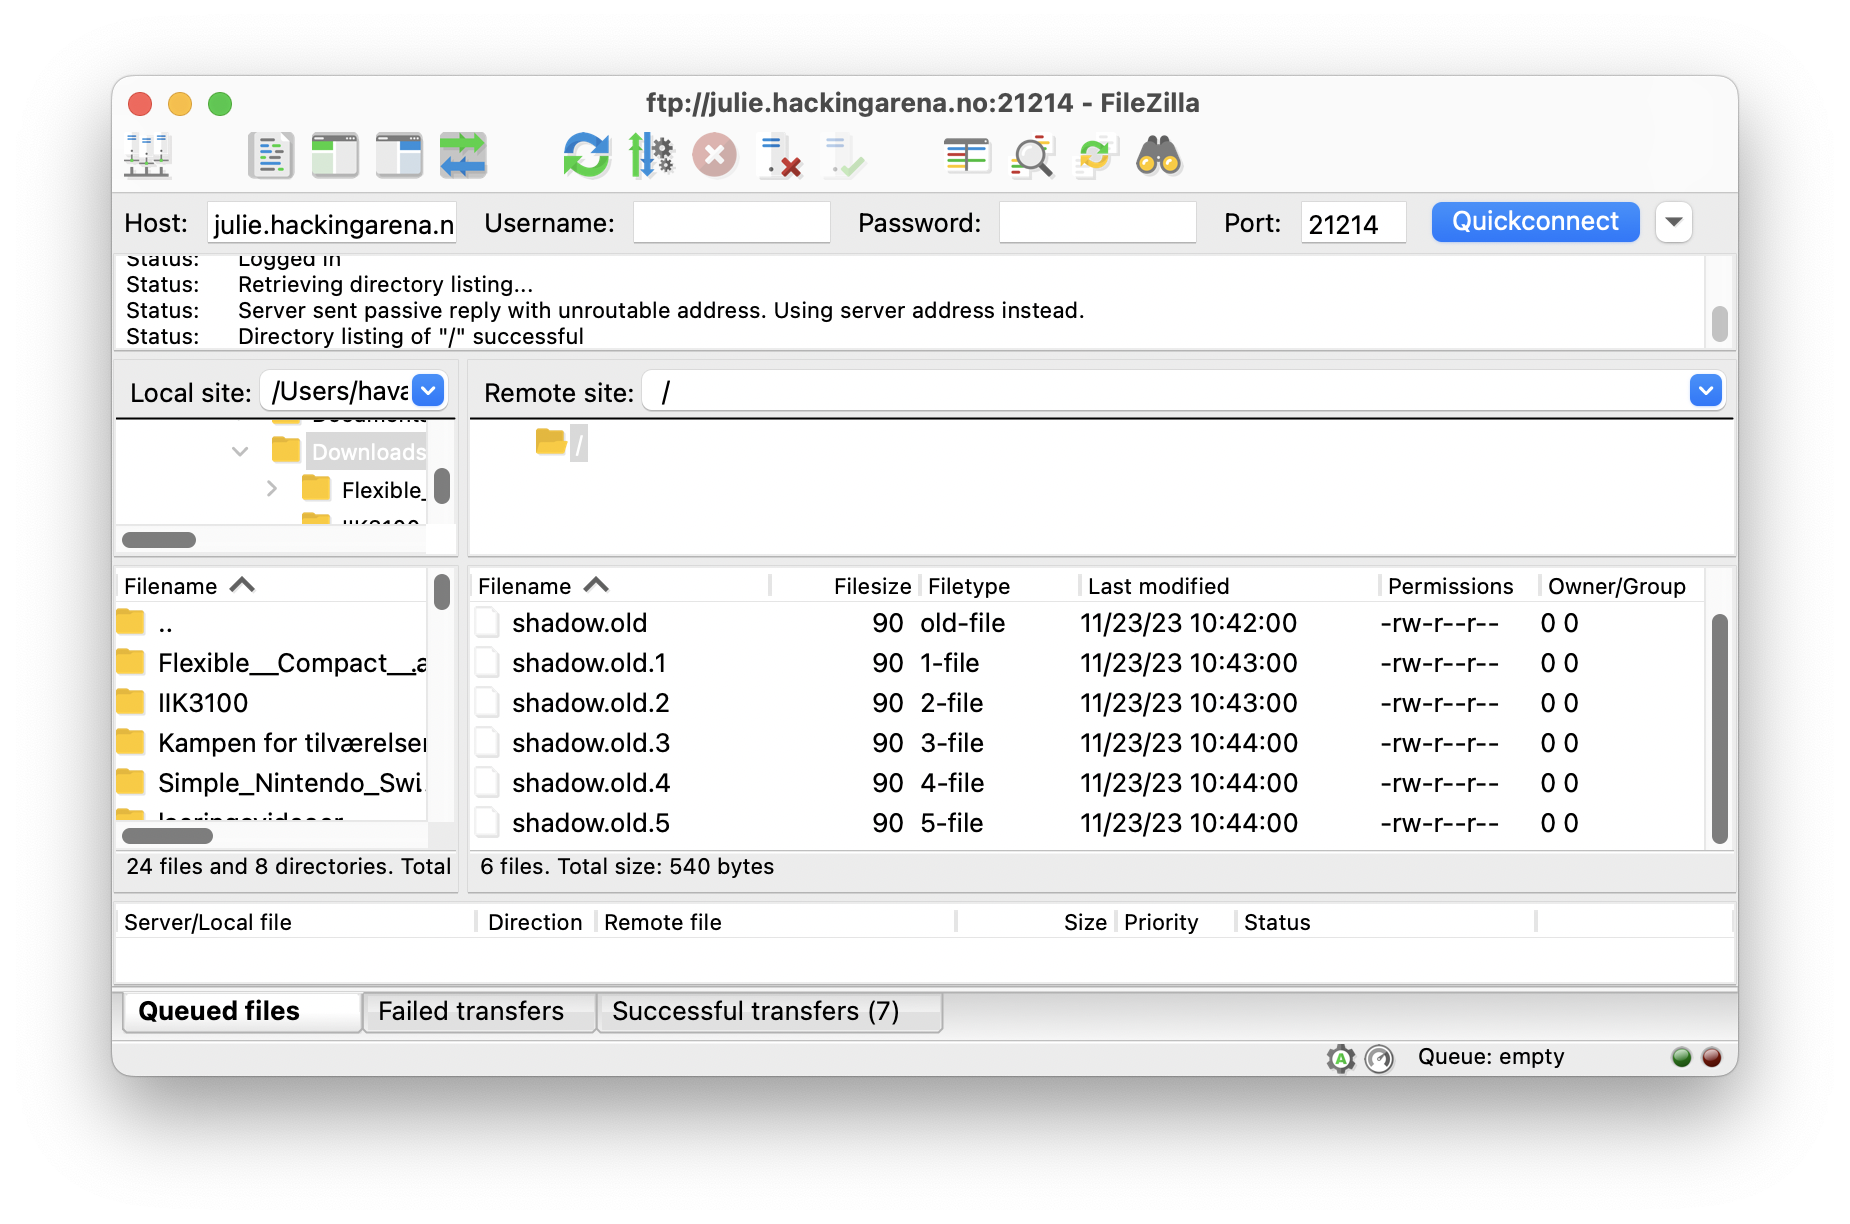
\includegraphics[width=13cm]{img/Get in touch with services/5th challenge/Screenshot 2023-11-24 at 14.00.01.png}
\end{center}

Opening the files revealed what looked like some hashed login credentials. I used \url{https://www.dcode.fr/md5-hash} to crack the hashes and found the following credentials:

\begin{alltt}
> shadow.old
lou:Mary
> shadow.old.1
lou:Sandra
> shadow.old.2
lou:Tina
> shadow.old.3
lou:Rita
> shadow.old.4
lou:Monica
> shadow.old.5
lou:Mary
\end{alltt}

Given the six names and the intro text to the task I connected that this was a reference to the song \textit{Mambo No. 5} by Lou Bega. Looking at the chorus of the song I found one of the names that was not used in the hashes, \texttt{Jessica}.

\begin{alltt}
[Chorus]
A little bit of Monica in my life
A little bit of Erica by my side
A little bit of Rita's all I need
A little bit of Tina's what I see
A little bit of Sandra in the sun
A little bit of Mary all night long
A little bit of \textbf{\emph{Jessica}}, here I am
A little bit of you makes me your man (Ha!)
\end{alltt}

I then logged in to the FTP server with the username \texttt{lou} and the password \texttt{Jessica} and found the flag file.

\begin{center}
    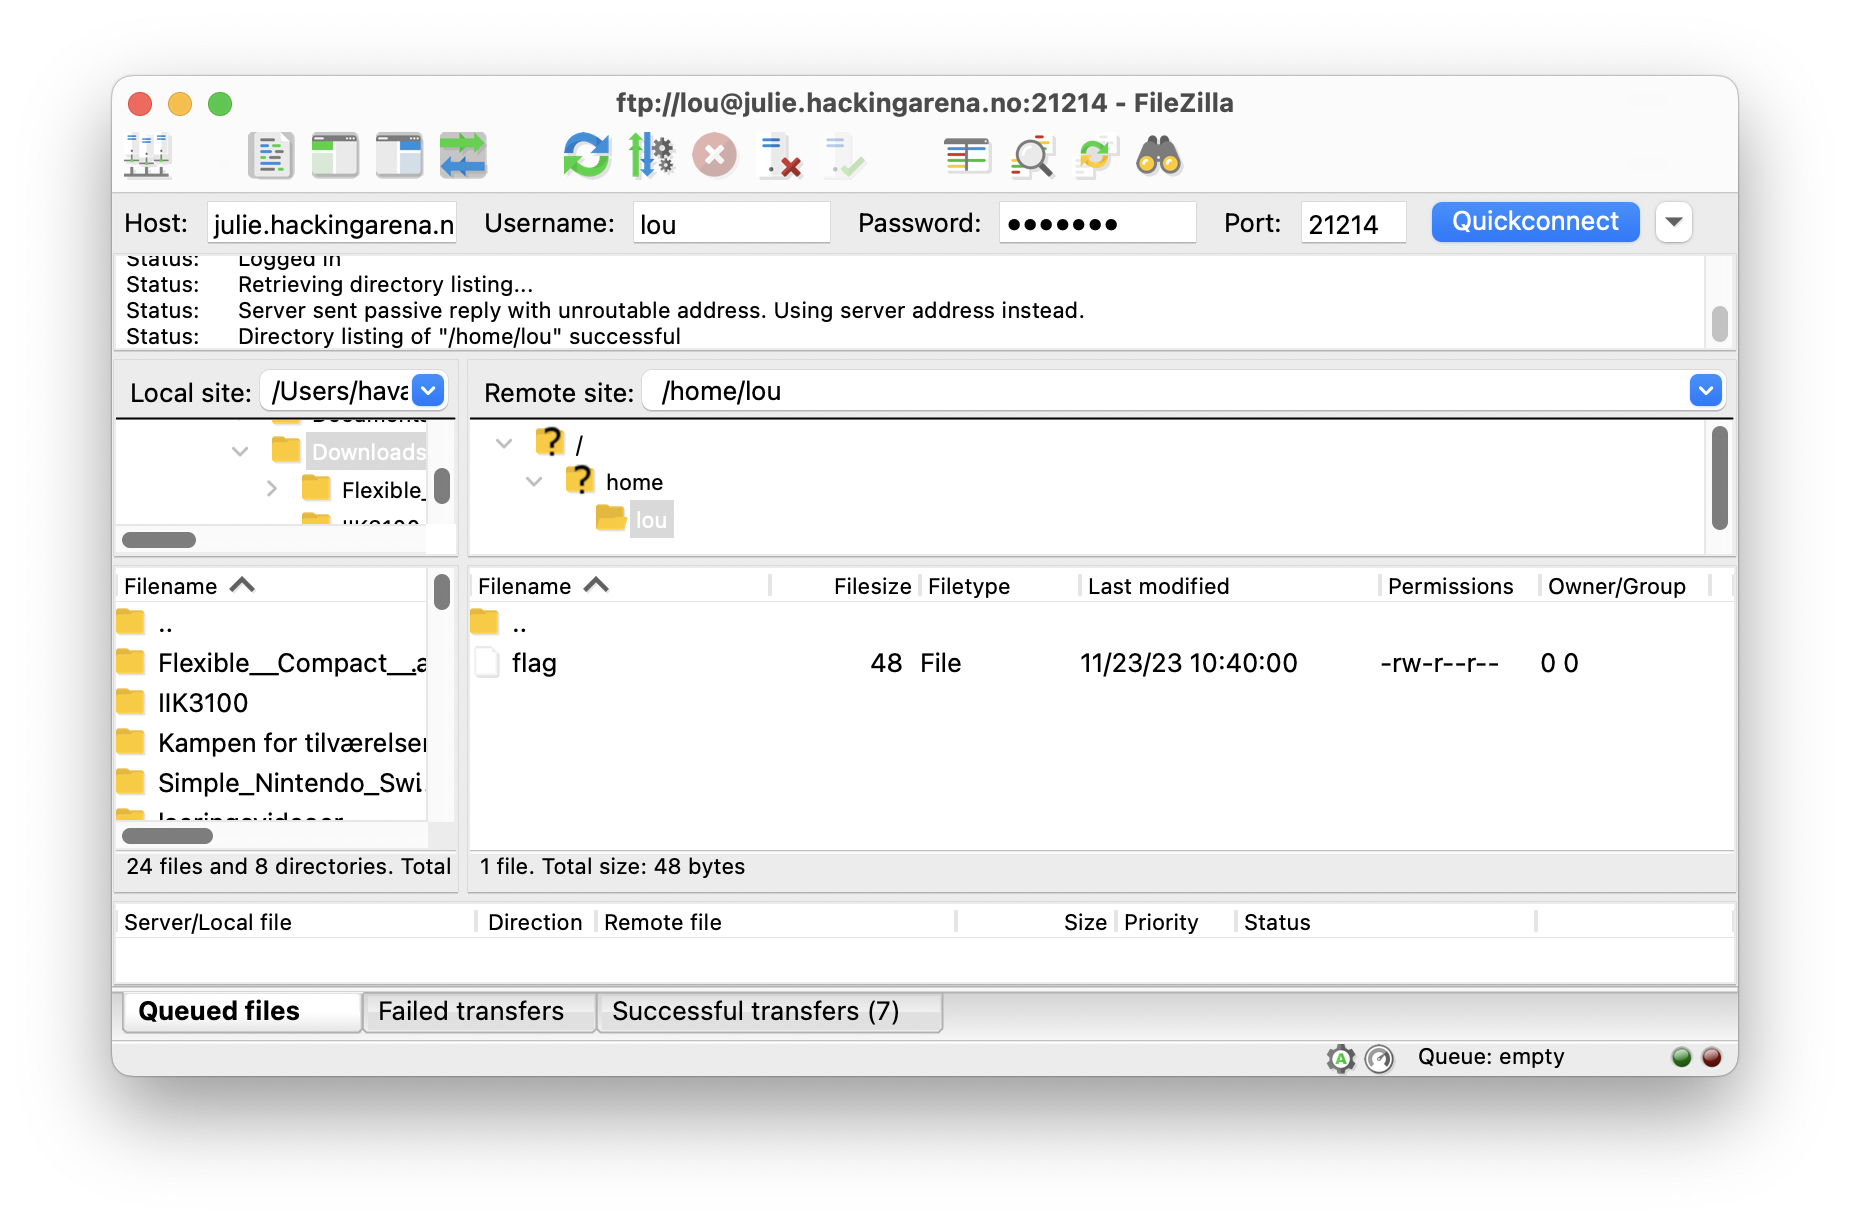
\includegraphics[width=13cm]{img/Get in touch with services/5th challenge/Screenshot 2023-11-24 at 14.00.21.png}
\end{center}

The flag was \texttt{Hacking-Arena\{Everybody\_in\_come\_on\_let's\_flag\}\}}.
\section{Web hacking}

\subsection{Unicorn 1 (100p)}
\subsection{Tricky login (100p)}

\newpage
\subsection{Order a Unicorn (100p)}
\addtocounter{points}{100}
Do you want to order a Unicorn?
\\Well, let's try it: \url{http://julie2.hackingarena.no:804}

\textbf{Solution:}\\
First I used the php filter \texttt{php://filter/convert.base64-encode/resource=index.php} to get the base64 encoded source code of the index.php file. 

\begin{center}
    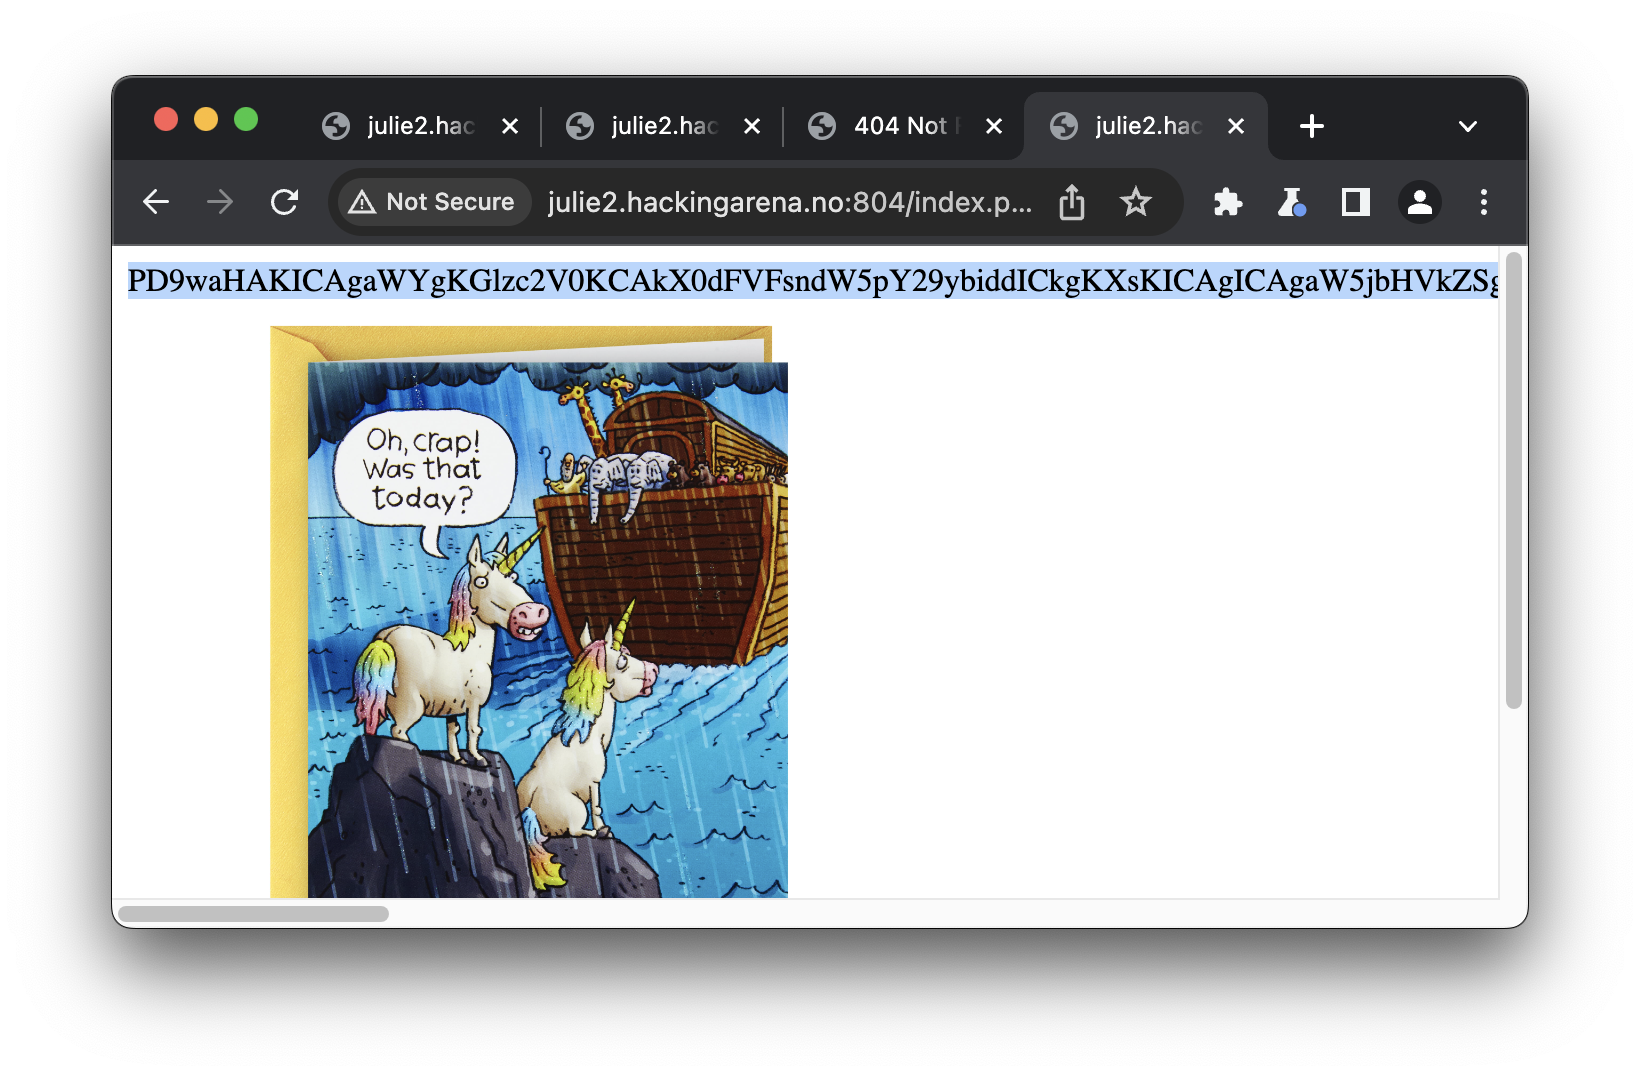
\includegraphics[width=12cm]{img/Web hacking/Order a Unicorn/Screenshot 2023-11-24 at 12.54.35.png}
\end{center}

Then I decoded it and found the following code:

\begin{center}
    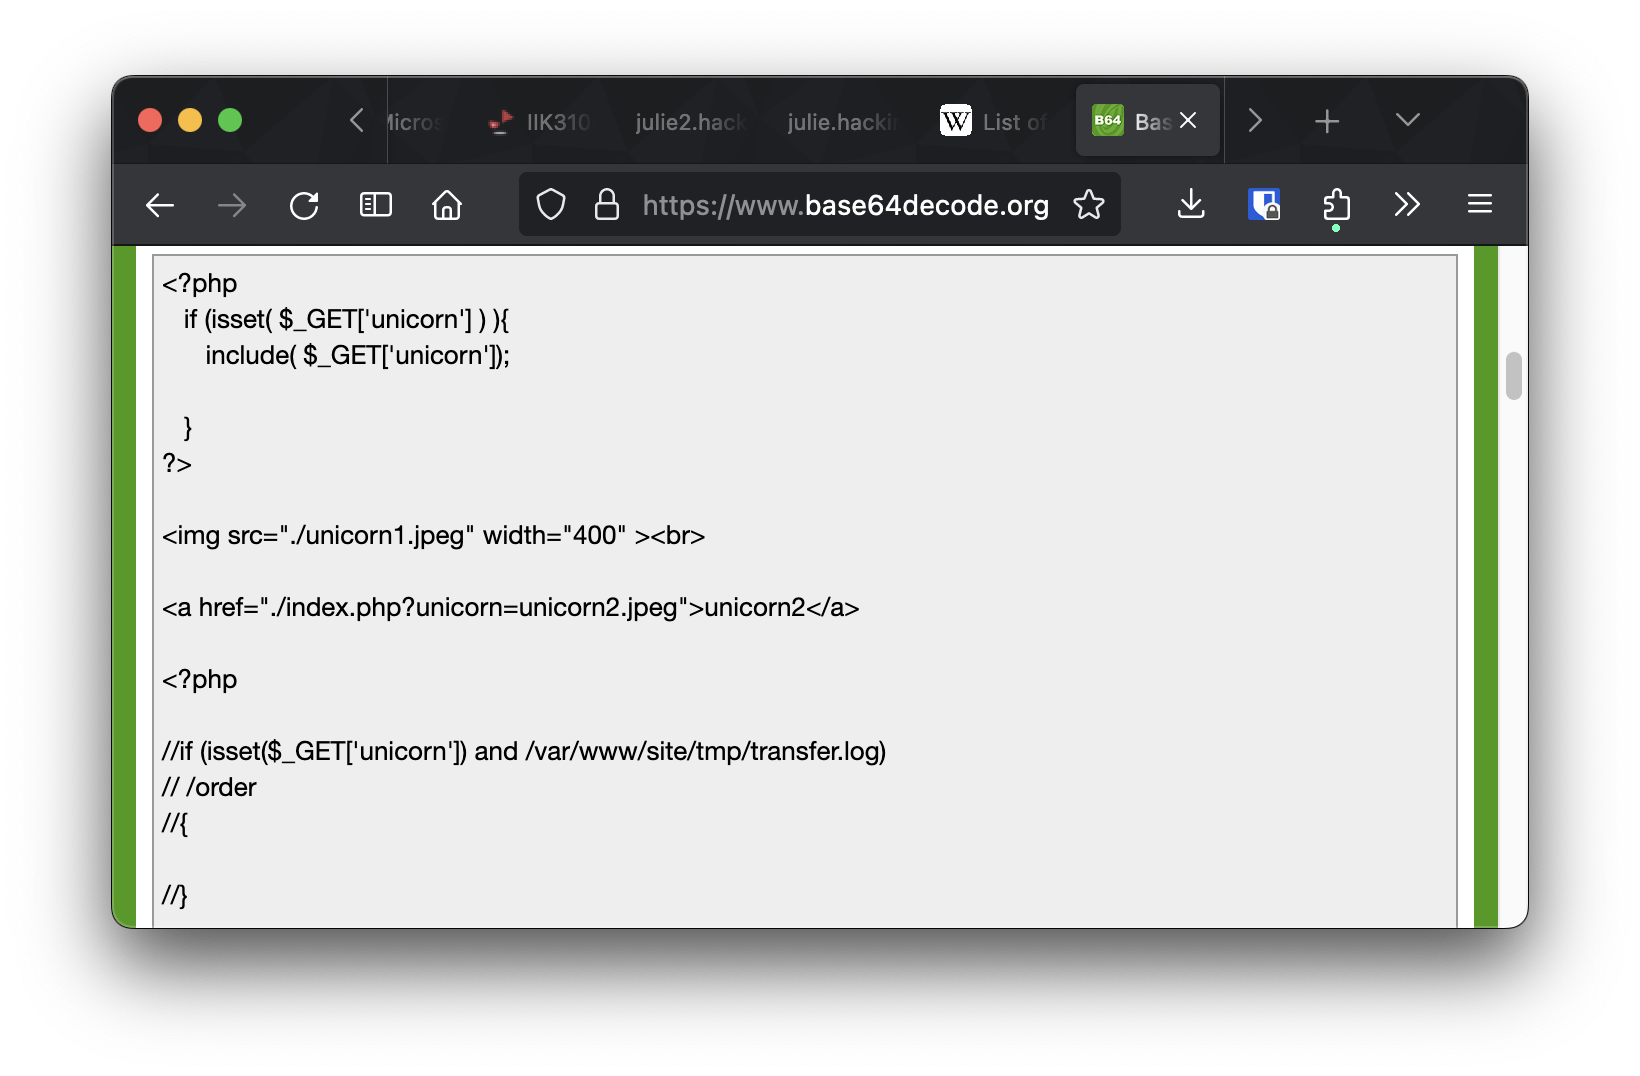
\includegraphics[width=12cm]{img/Web hacking/Order a Unicorn/Screenshot 2023-11-24 at 12.54.54.png}
\end{center}

I then looked at the \texttt{/var/www/site/tmp/transfer.log} that was revealed by the source code and found the following stride payment records:

\begin{center}
    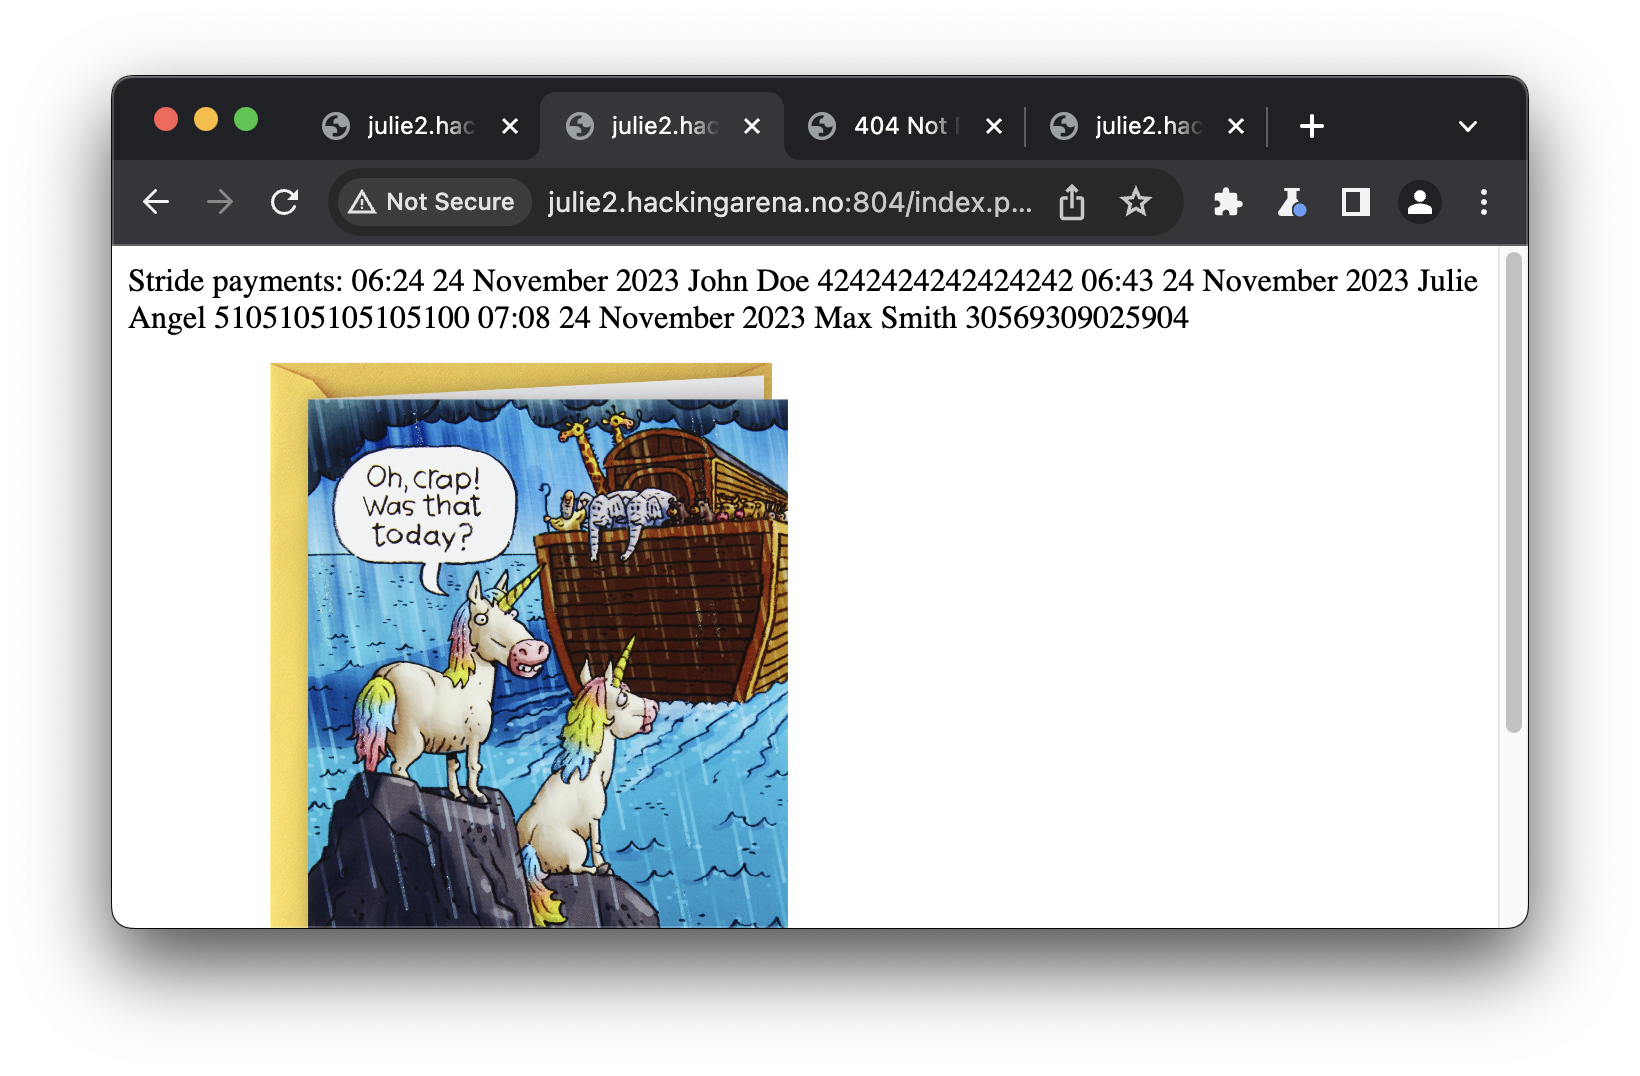
\includegraphics[width=14cm]{img/Web hacking/Order a Unicorn/Screenshot 2023-11-24 at 12.55.13.png}
\end{center}

I then when to the \texttt{/order} page and tried to order a unicorn with the card numbers from the stride payment records. But since none of them worked I started looking for example card numbers online and found a list from paypal test credit cards.

\begin{center}
    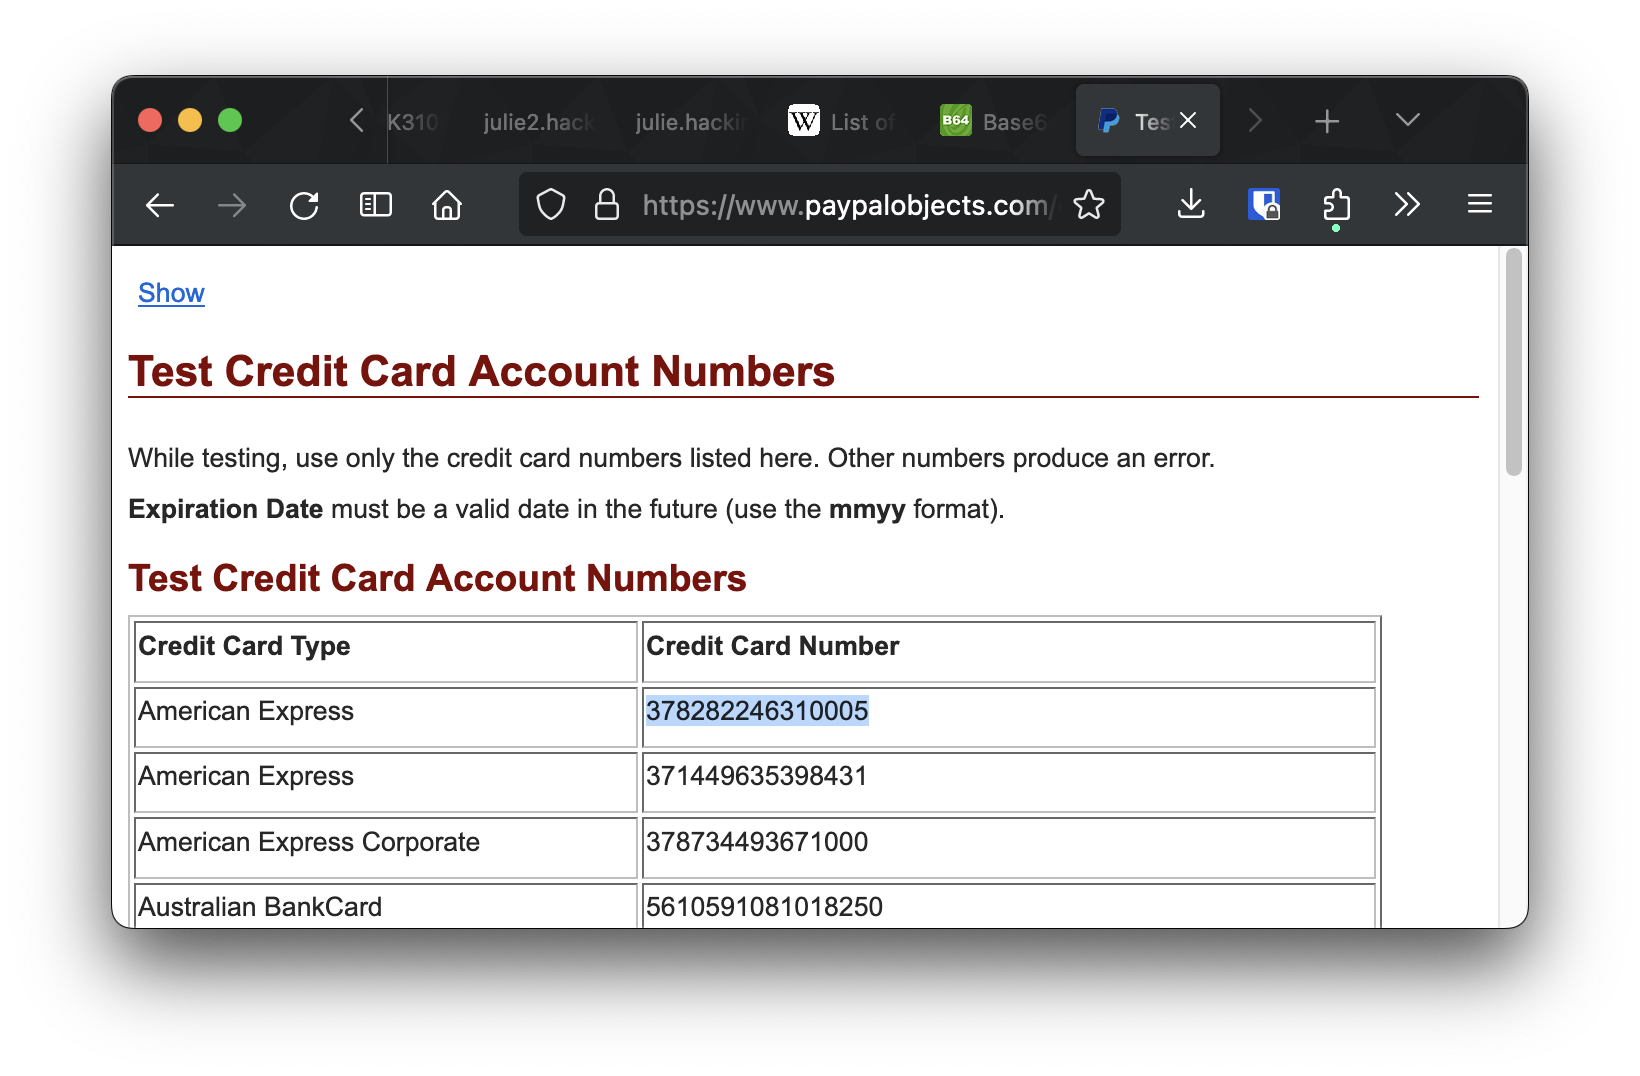
\includegraphics[width=15cm]{img/Web hacking/Order a Unicorn/Screenshot 2023-11-24 at 12.55.43.png}
\end{center}

I then tried to order a unicorn with the card number \texttt{378282246310005}...

\begin{center}
    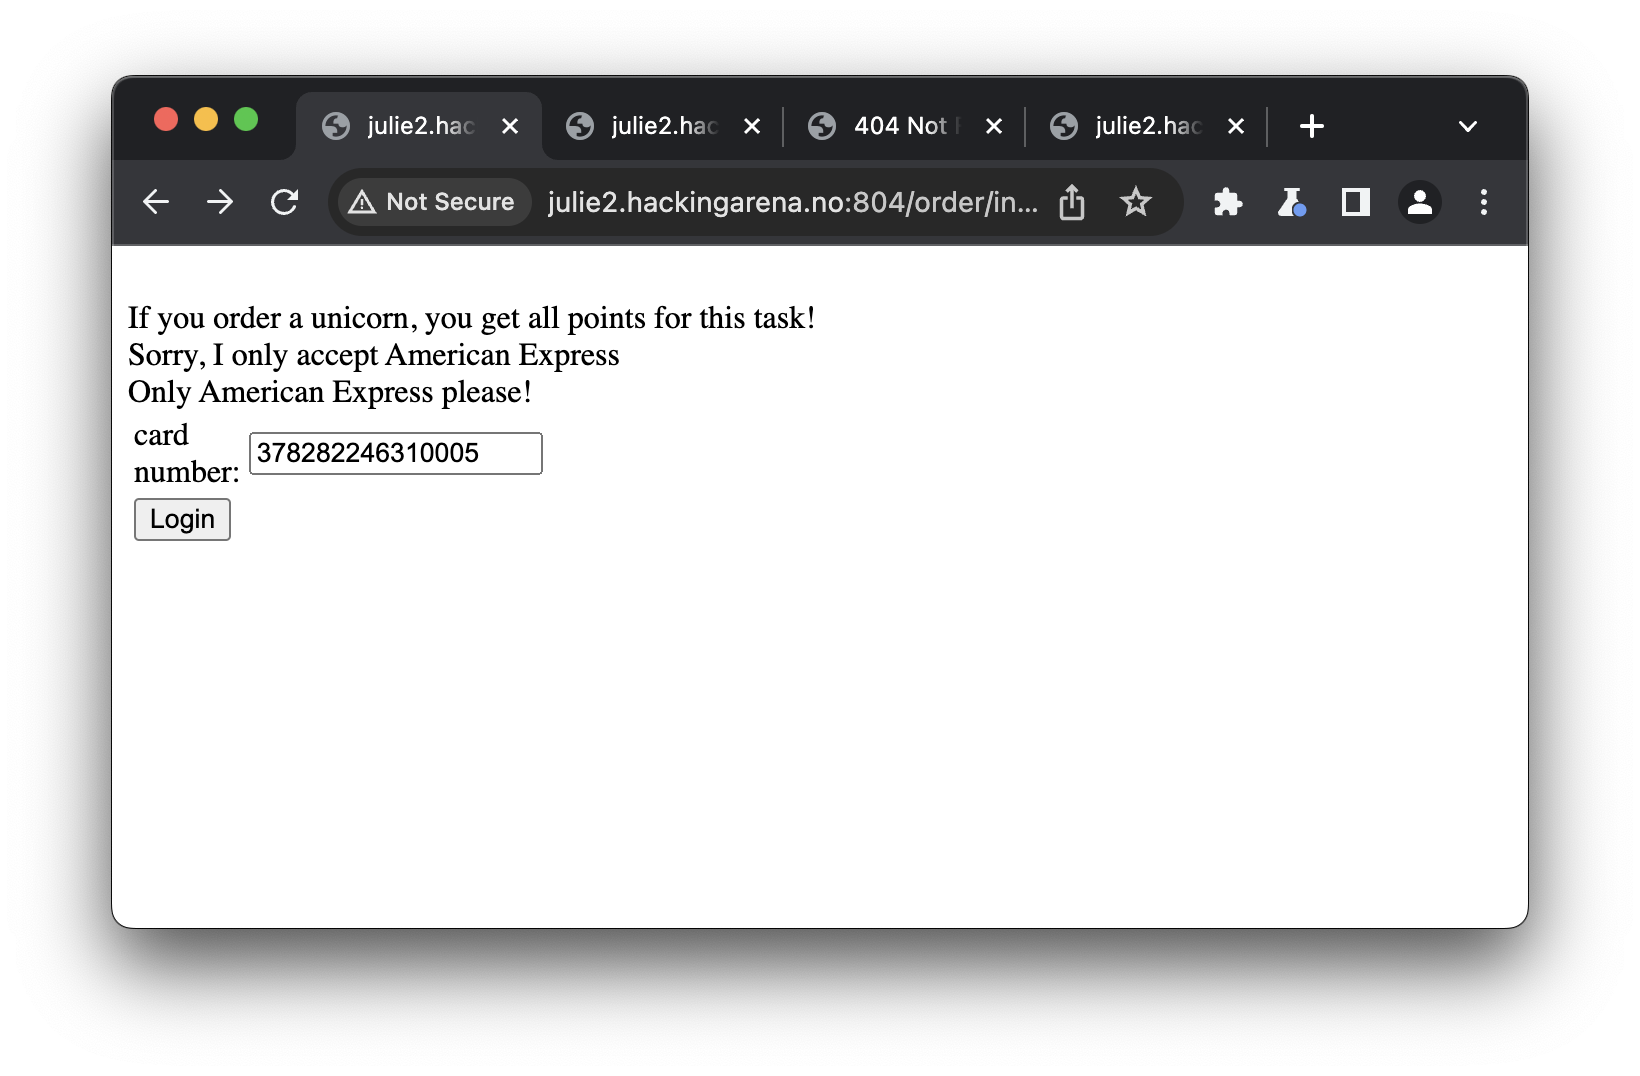
\includegraphics[width=15cm]{img/Web hacking/Order a Unicorn/Screenshot 2023-11-24 at 12.55.22.png}
\end{center}

...and got the flag.

\begin{center}
    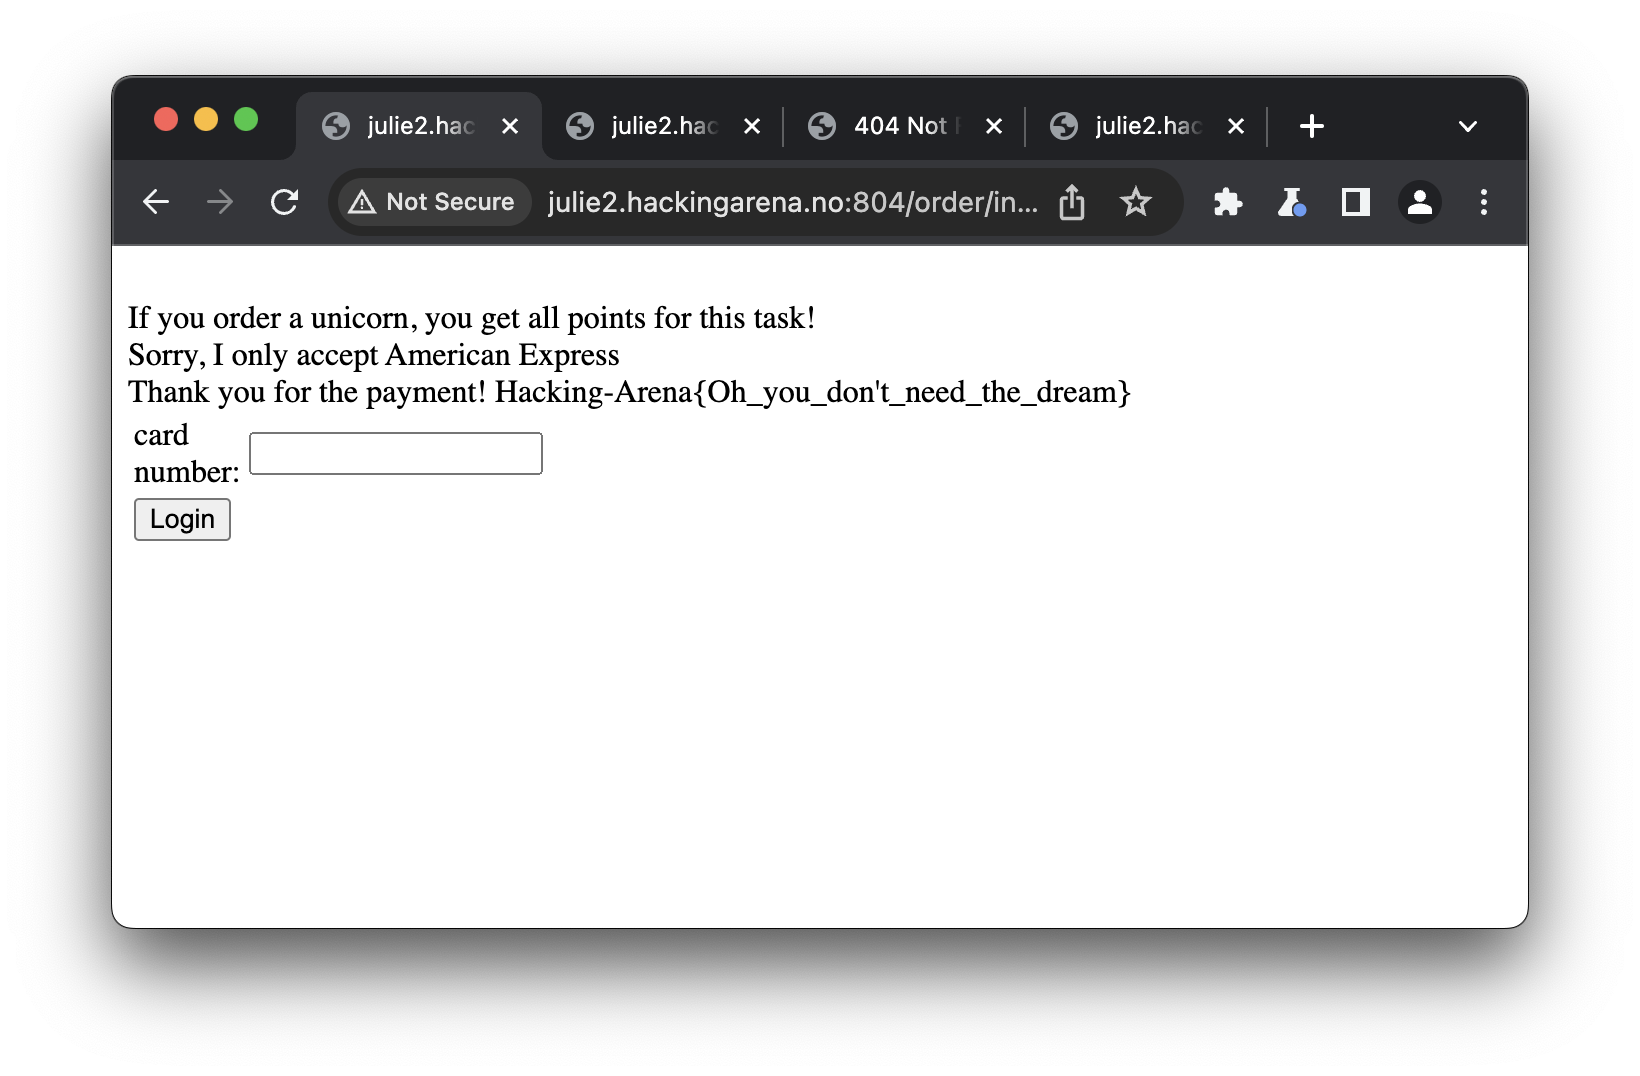
\includegraphics[width=15cm]{img/Web hacking/Order a Unicorn/Screenshot 2023-11-24 at 12.55.26.png}
\end{center}
\newpage
\section*{}
\addcontentsline{toc}{section}{Total points: \arabic{points}p}
\begin{center}
    \topskip0pt
    \vspace*{\fill}
    this page is intentionally left blank
    \vspace*{\fill}
\end{center}
\pagenumbering{gobble}

% \printbibliography[heading=bibintoc] % LAGER BIBLIOGRAFI
\end{document}
